\documentclass{article}
\usepackage[slovak]{babel}
\usepackage{graphicx}
\usepackage[top=1in, bottom=1.25in, left=1.25in, right=1.25in]{geometry}
\begin{document}
\noindent
\large
Adam Jenča\\
Tercia A\\
SŠ Novohradská, Bratislava\\
Príklad Z9-I-6\\
\vskip 5mm \noindent
\begin{center}
	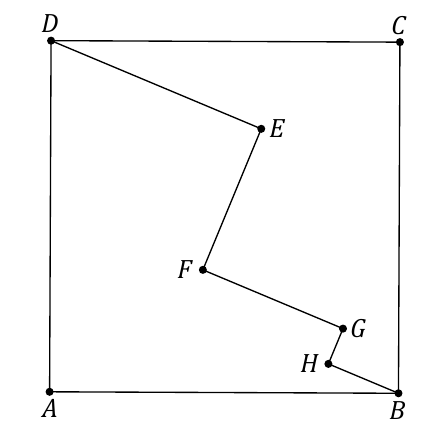
\includegraphics[scale=0.3]{xetex/imagery/squeer}
\end{center}
\vskip 5mm
Keďže sú uhly $DEF$, $EFG$, $FGH$ a $GHB$ pravé, môžeme lomenú čiaru preusporiadať na odvesny($i$, $j$) pravouhlého trojuholníka s preponou $DB$ ($k$). Jednu z odvesien($i$) budú tvoriť úsečky $DE$ , $FG$, a $HB$ , pričom druhú($j$) budú tvoriť úsečky $EF$ a $GH$. Vieme,že $i = |DE| + |FG| + |HB| = 6cm + 4cm + 2cm = 12cm$ a $j = |EF| + |GH| = 4+1=5cm$.\\
Teraz si zistíme štvorec uhlopriečky $DB$($k$):
$$
k^2 = i^2 + j^2 = 12^2 + 5^2 = 169cm^2
$$
Keďže $ABCD$ je štvorec, vieme že $k^2 = 2a^2$. Preto
$$
S_{ABCD} = a^2 = \frac{k^2}{2} = \frac{169cm^2}{2} = 84,5cm^2
$$
\textbf{Obsah štvorca je teda $\mathbf{84,5cm^2}$}
\end{document}
